\chapter{Case setup}
\section{A test case}
With the help of the OpenFOAM tutorial case study, a test case was set up
for the simulation of multiphase flow over a NACA0012 hydrofoil. The geometry is from a compressible flow tutorial 
where  k-$\omega$ sst turbulence model was adopted. The $\textit{blockMeshDict}$ of that tutorial is relevant for the thesis since it helps 
to tune the mesh based on requirement. To set up the case folders for multiphase simulation, another case study 
tutorial was used: multiphase/interFoam/RAS/propeller. The mass transfer model used in the tutorial is 
Schnerr-Sauer, that relevant for  thesis it was explained in (chapter 2 section 2.2.4) and also the tutorial assists with setting up 
the 3 folders to run the simulation properly. The essential file from the tutorials are copied in the working directory.
files from the tutorials. The case setup of the working directory contains three folders 
$\textit {0/, constant/, and system/}$, with slight modification  in all three 
of them as outlined below.
\section{Computational domain}
The flow field around the hydrofoil is modeled in two-dimensional.
\begin{figure}[H]
    \centering
    \includegraphics[scale=0.4]{blockMesh.png}
    \caption{Schematic representation of flow field around 2D NACA0012 hydrofoil with boundary condition}
    \label{fig:fig16}
\end{figure}
The transformation from 2D to 3D performed in domain of  $\textit{blockMeshDict}$ by adding ymax=0.45 and ymin=-0.45 which is in span wise direction.
\begin{figure}[H]
    \centering
    \includegraphics[scale=0.4]{AOA83Dblockmesh}
    \caption{Schematic representation of flow field around 3D NACA0012 wing }
    \label{fig:fig17}
\end{figure}
\subsection{Boundary and initial condition}
The boundary condition and parameters of work condition  are taken from the reference
\cite{Zhao2021} which is stated below:
\begin{table}[h]
    \centering
    \begin{tabular}{|c|c|}
    \hline
        hydrofoil & Wall \\
    \hline
        inlet & Velocity \\ 
    \hline
       outlet & Pressure  \\
    \hline
       top and bottom & Symmetry \\
   \hline
    \end{tabular}
    \caption{Boundary condition}
    \label{tab:BC}
\end{table}
The parameter of working condition is stated below:
\begin{table}[h]
    \centering
    \begin{tabular}{|c|c|}
    \hline
        Velocity(U) & 5 m/s \\
    \hline
        Cavitation number ($\sigma$) & 0.8 \\ 
    \hline
     Turbulence kinetic energy(k) & 0.0185 $m^2$/$s^2$ \\
    \hline
    Specific dissipation rate($\omega$) & 621.626 $s^{-1}$ \\
    \hline
    pressure($P_v$) & 9358.6848 N/${m}^2$\\
    \hline
    Reference pressure($P_{out}$) &  0.203e5 N/${m}^2$ \\
    \hline
    Chord length(C) & 100 mm \\
    \hline
    Angle of attack($\alpha$) & ${3.2}^{\circ}$ to ${8}^{\circ}$ \\
   \hline
    \end{tabular}
    \caption{parameters of work condition}
    \label{tab:PC}
\end{table}
\section{Grid study}
In this thesis, the influence of mesh size was discussed. Three types of mesh were analyzed to 
determine the appropriate mesh size for numerical simulation. It was clear that the force coefficient increased when
mesh size was small. It can be seen from the verification and validation results that the value of numerical 
uncertainty is larger than the comparison error. Thus, the calculated results are in agreement, but there 
is not enough evidence to confirm their accuracy. The grid study is discussed in the table below, which takes the AOA $5^{\circ}$ degree into account. 
\begin{table}[h]
\centering
\begin{tabular}{|l|l|l|l|l|l|}
\hline
 \rowcolor{gray!20}Grid no& No of cells & No of faces &No of points  & Cl & Cd \\ \hline
Grid A & 16000 & 64240 & 32480  & 0.72 & 0.028 \\ \hline
 Grid B& 21600 & 86690 & 43780 & 0.68 & 0.027 \\ \hline
Grid C & 38500  & 154390 &77780  & 0.59 & 0.021 \\ \hline
\end{tabular}
\caption{Grid study of  AOA $5^{\circ}$}
\label{fig: fig16}
\end{table}
\begin{figure}[H]
    \centering
    \includegraphics[scale=0.4]{gridstudy.png}
    \caption{Grid lines in coarse mesh over view}
    \label{fig:fig17}
\end{figure}
\section{Case folder setup}
\subsection{0 Folder}This folder contains the working parameters  at the boundaries for the initial time step, such 
as velocity as ${\textit {U}}/$ which is a reference velocity, ${\textit{p}}_{{\textit {\_rgh}}}/$  
reference pressure, ${\textit {omega}}/$ specific dissipation rate, ${\textit {k}}/$ 
turbulence kinetic energy, ${\textit {nut}}/$, ${\textit {alpha.water}}/$ vapour fraction 
respectively. In order to include the angle of attack of the hydrofoil with respective to the incoming flow it is better to specify the velocity as 
$V_x$=V$cos \alpha$ and $V_z$=$V sin \alpha$(normal direction is in z direction). The internalField and 
boundaryField of each files in the $0/$ folder are stated below:\\ 
\begin{table}[h]
\centering
\begin{tabular}{|l|l|l|l|l|}
\hline
 \rowcolor{gray!20}      PATCH           &FIELD  & UNITS & TYPE &VALUE \\ \hline
\multirow{6}{*}{inlet} & U & m/s & fixed value  & 5  \\ \cline{2-5} 
                  &P  & Pa & zero gradient &- \\ \cline{2-5} 
                  &$\omega$  & $s^{-1}$ &fixed value  & 621.626 \\ \cline{2-5} 
                  & k & $m^2$/$s^2$ & fixed value & 0.0185 \\ \cline{2-5} 
                  & nut & $m^2$/s & zero gradient & 0 \\ \cline{2-5} 
                  &alpha.water  & - &fixed value  & 1 \\ \hline
\multirow{6}{*}{outlet} & U & m/s & zero gradient &-  \\ \cline{2-5} 
                  & P & Pa & fixed value  & 0.203e5 \\ \cline{2-5} 
                  & $\omega$ & 1/s & fixed value & 621.626 \\ \cline{2-5} 
                  &  k& $m^2$/$s^2$ & fixed value & 0.0185 \\ \cline{2-5} 
                  & nut & $m^2$/s & fixed value & 0 \\ \cline{2-5} 
                  & alpha.water & - &fixed value & 1 \\ \hline
\end{tabular}
\caption{Boundary condition}
\end{table}





\subsection{Constant folder}
This folders includes 4 files namely $\textit{g}/$, $\textit{momentum transport}/$, 
$\textit{phaseChangeProperties}/$, $\textit{transportProperties}/$ and two other subfolderwhich are called  geometry 
and polyMesh. In $\textit{geometry}/$, the NACA0012.obj is present. This file which helps to run the
$\textit{blockMesh}$ command in the working directory to generate the $\textit{polyMesh}/$ folder in the 
constant folder. This folder contains some files such as $\textit{boundary}/$, $\textit{face}/$, $\textit{neighbor}/$, 
$\textit{owner}/$, $\textit{points}/$.\\The $\textit{momentumTransport/}$ file is the place for the declaration 
of turbulence model.
\begin{table}[h]
\centering
\begin{tabular}{|lll|}
\hline
\rowcolor{gray!20}\multicolumn{3}{|l|}{momentumTransport}                            \\ \hline
\multicolumn{1}{|l|}{simulationType } & \multicolumn{1}{l|}{RAS} & model:          kOmegaSST \\ \hline
\end{tabular}
\caption{Parameters in momentumTransport}
\label{tab:PC}
\end{table}








\begin{table}[h]
\centering
\begin{tabular}{|ccc|}
\hline
\rowcolor{gray!20}\multicolumn{3}{|c|}{PhaseChangeProperties}                            \\ \hline
\multicolumn{1}{|c|}{phaseChangeModel} & \multicolumn{1}{c|}{SchnerrSauer} & SchnerrSauerCoeffs on \\ \hline
\multicolumn{1}{|c|}{pSat(saturation vapor pressure)} & \multicolumn{2}{c|}{9358.6848 $N/{m^2}$}    \\ \hline
\end{tabular}
\caption{Parameters in phaseChangeProperties}
\label{tab:PC}
\end{table}







\begin{table}[h]
\centering
\begin{tabular}{|ll|}
\hline
\rowcolor{gray!20}\multicolumn{2}{|l|}{transportProperties}    \\ \hline
\multicolumn{1}{|l|}{phases} &water vapour  \\ \hline
\multicolumn{1}{|l|}{pSat} & 9358.6848 $N/{m^2}$\\ \hline
\multicolumn{1}{|l|}{sigma(cavitation number) } & 0.8 \\ \hline
\end{tabular}
\caption{Parameters in transportProperties}
\label{tab:PC}
\end{table}












The $\textit{phaseChangeProperties/}$ file is the place for the declaration of mass transfer model and saturation vapor pressure. The
$\textit{transportProperties}/$ is the place to declare the phase of a mixture, its properties, as well as the cavitation number.
\subsection{System folder}
This folder contains files such as  $\textit{blockMeshDict}/$, $\textit{controlDict}/$, $\textit{decomposeParDict}/$, 
$\textit{extrudeMeshDict}/$, $\textit{fvScheme}/$, $\textit{fvSolution}/$. Tune mesh based on requirements aids mesh grading in the $\textit{blockMeshDict}/$.
By specifying ymin=-0.45 and ymax=0.45 in the domain of  $\textit{blockMeshDict}/$, one can go from 2D to 3D.   \\
\subsubsection{Time step control}
The courant number affects the reliability and stability of the unstable flow simulation. The maxCo should 
be set around 5 in the $\textit{controlDict}/$ file. Based on the mesh adopted deltaT of 1e-5 s is sufficient to satisfy the condition. Note that cavitating flow calculations 
should always be initiated from a flow field. When cavitation is toggled on, simulation must be restarted from the 
current flow field.\\
\subsubsection{Discretisation schemes}
In OpenFOAM, the free surface treatment does not account for turbulence. All free surface simulations can be viewed 
as direct numerical simulations (DNS). Therefore there is a high requirement for the mesh resolution of the interface. 
The solver uses the multidimensional universal limiter for explicit solutions (MULES) to maintain the boundedness of 
the phase fraction, regardless of the underlying numerical scheme, mesh structure, etc. The choice of schemes for 
convection is therefore not restricted to those that are strongly stable or bounded, e.g. upwind differencing.\\
\subsubsection{Solution and algorithm control}
The $\textit{fvSolution/}$ file controls the equation solvers, tolerances and algorithms. 
In the first subdictionary, solver, each linear-solver used for each discretized equation is specified. This is achieved by
specifying the solver of each variable being solved, in this case: pcorr (pressure corrector), p$\_$rgh, p$\_$rghFinal
(the final value of pressure after the correction), $(U|k|omega)$, $(U|k|omega)Final$ and alpha.water. The variable name is followed by the
solver name and a dictionary containing the parameters that the solver uses. The pressure variables are solved with the aid of solver GAMG 
and smoother DICGaussSeidel(Diagonal Incomplete Cholesky), velocity and turbulence quantities are solved using a  
smoothSolver and smoother symGaussSeidel, and volume fraction alpha.water by way of MULES. The tolerance, and ratio of 
current to initial residuals, relTol, are specified afterward. The solver stops if one of the two tolerances falls 
beneath the targeted value. The precept of GAMG is to generate a quick solution on a mesh with a small number of cells, 
map this solution onto a finer mesh, and use it as an initial guess to obtain a correct solution on the fine mesh.\\
\begin{figure}[H]
    \centering
    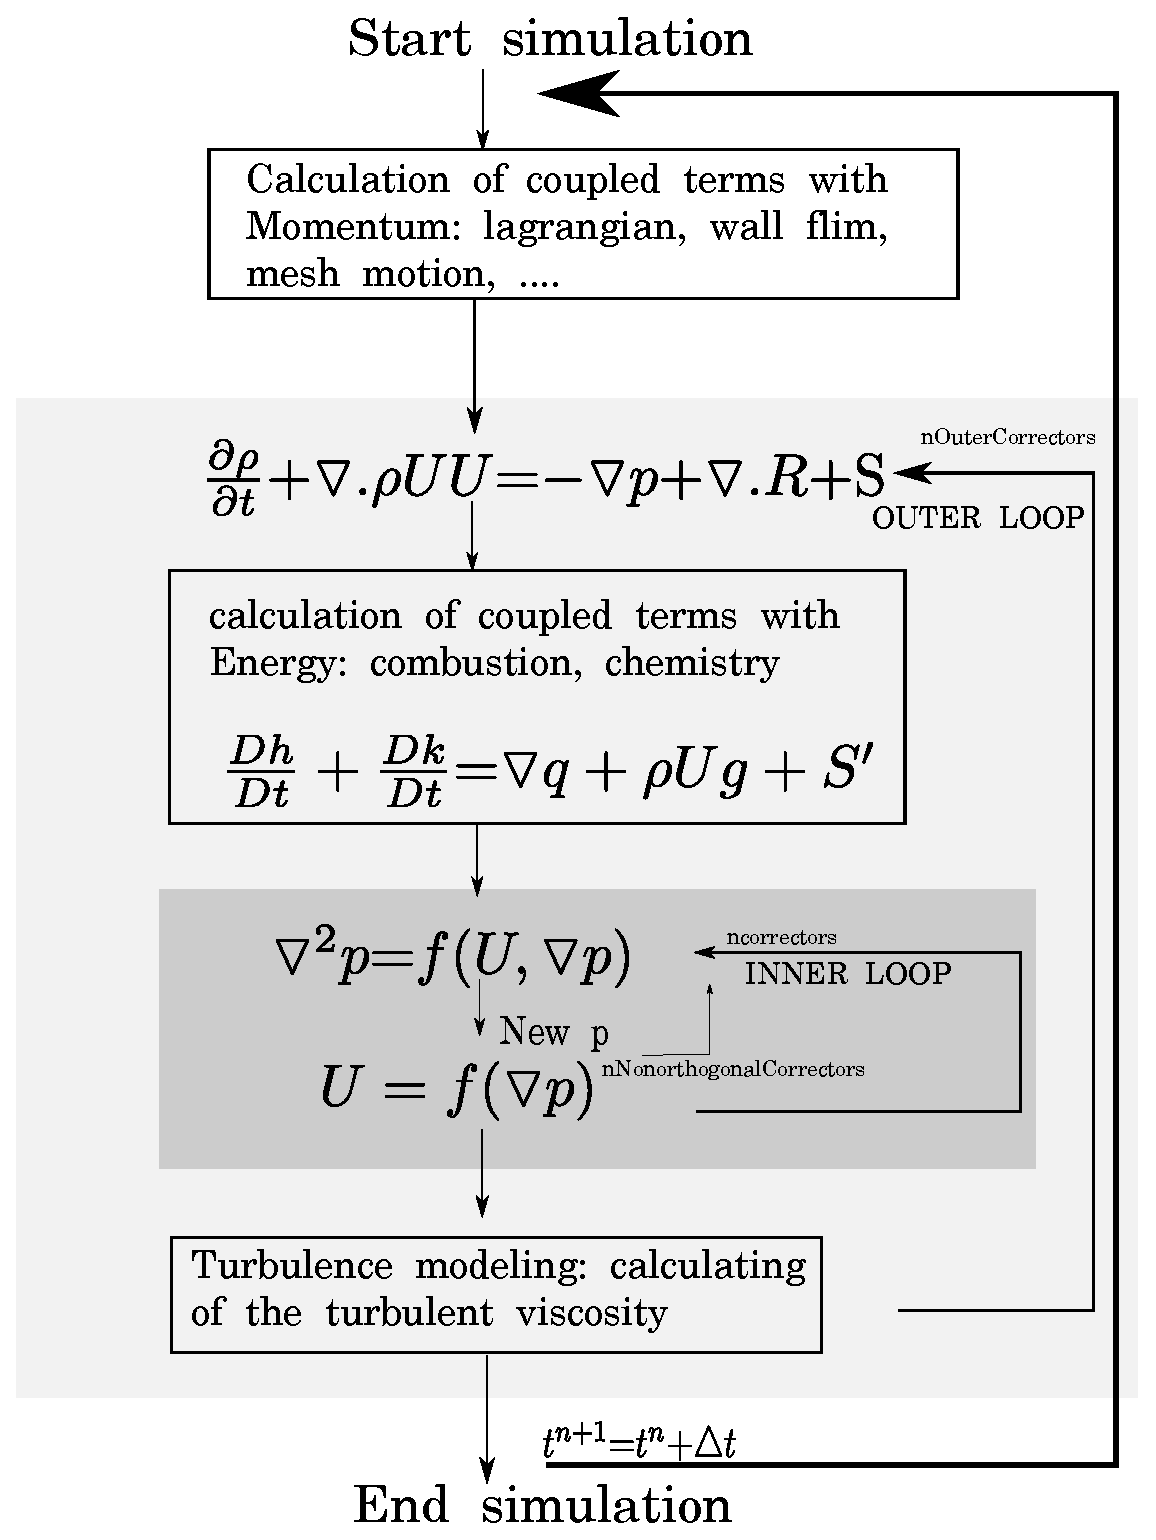
\includegraphics[scale=0.4]{PIMPLEflowchart}
    \caption{rhoPimpleFoam-based solvers}
    \label{fig:fig16}
\end{figure}

In OpenFOAM, any compressible flow solver is usually based on PIMPLE, which is an algorithm of iterative procedures 
for solving equations for velocity and pressure of unsteady problems. PIMPLE is an unsteady, transient SIMPLE.
The number of correctors is specified by the keyword nCorrectors which should be greater than 1. The number of non-orthogonal correctors is specified by the 
nNonOrthogonalCorrectors keyword to account for mesh non-orthogonality which should be greater than 1. 
In the thesis, nOuterCorrectors should be set to 3, nCorrectors to 1, and nNonOrthogonalCorrectors to 0.
\subsection{Postprocessing}
To validate the force in the x and z direction it is better to use the force function object. This forces function
object generates hydrodynamic force and moment data for surfaces. The forces comprise normal pressure
and tangential viscous contributions. The forces obtained from the postprocessing are used for calculating the
Cl and Cd. The basic operation of the forces function object is cited in  $\textit{controlDict/}$ which comprises
mandatory entries stated below:\\
\begin{table}[h]
\centering
\begin{tabular}{|ll|}
\hline
\rowcolor{gray!20}\multicolumn{2}{|l|}{forces1}    \\ \hline
\multicolumn{1}{|l|}{type } &forces  \\ \hline
\multicolumn{1}{|l|}{libs} & libforces.so  \\ \hline
\multicolumn{1}{|l|}{patches} & hydrofoil(wall) \\ \hline
\end{tabular}
\caption{Forces function object}
\label{tab:PC}
\end{table}




Inorder to validate the term yplus the yPlus function object is used to computes the near wall $y^+$ for turbulence models
by using yPlus functions sub-dictionary in $\textit{system/controlDict}/$. It is better to use ${\#includeFunc}$ $yPlus$ 
in the function of $\textit{controlDict}/$.
The pressure function object provides to validate the total pressure coefficient. The following  mandatory entries are 
included in the function of $\textit{controlDict}/$ are stated below: 
 \begin{table}[h]
\centering
\begin{tabular}{|ll|}
\hline
\rowcolor{gray!20}\multicolumn{2}{|l|}{pressure1}    \\ \hline
\multicolumn{1}{|l|}{type } &pressure  \\ \hline
\multicolumn{1}{|l|}{libs} & libfieldFunctionObjects.so  \\ \hline
\multicolumn{1}{|l|}{mode} & totalCoeff \\ \hline
\end{tabular}
\caption{Pressure function object}
\label{tab:PC}
\end{table}























